\documentclass{article}
% successeur du package "graphics"
\usepackage{graphicx}
% pour pouvoir inclure des fichiers dont le chemin contient plus qu'un point,
% e.g. seam_carving.jl.pdf
\usepackage{grffile}
\usepackage{wrapfig}


\begin{document}
\textbf{Signature.} \verb|\includegraphics[options]{fichier}|
\vspace{10mm}


\begin{wrapfigure}[7]{o}{2cm}
  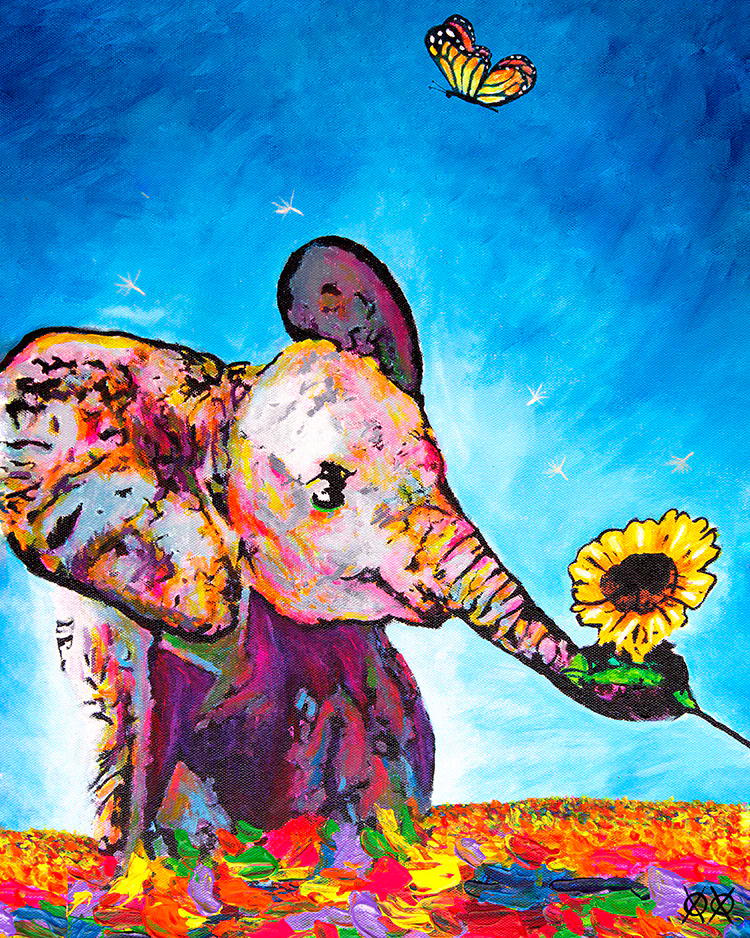
\includegraphics[width=15mm]{elephant.png}
\end{wrapfigure}
Pour inclure le dessin d'éléphant à la droite, j'ai fait comme indiqué dans le livre
\begin{verbatim}
  \begin{wrapfigure}[7]{o}{2cm}
    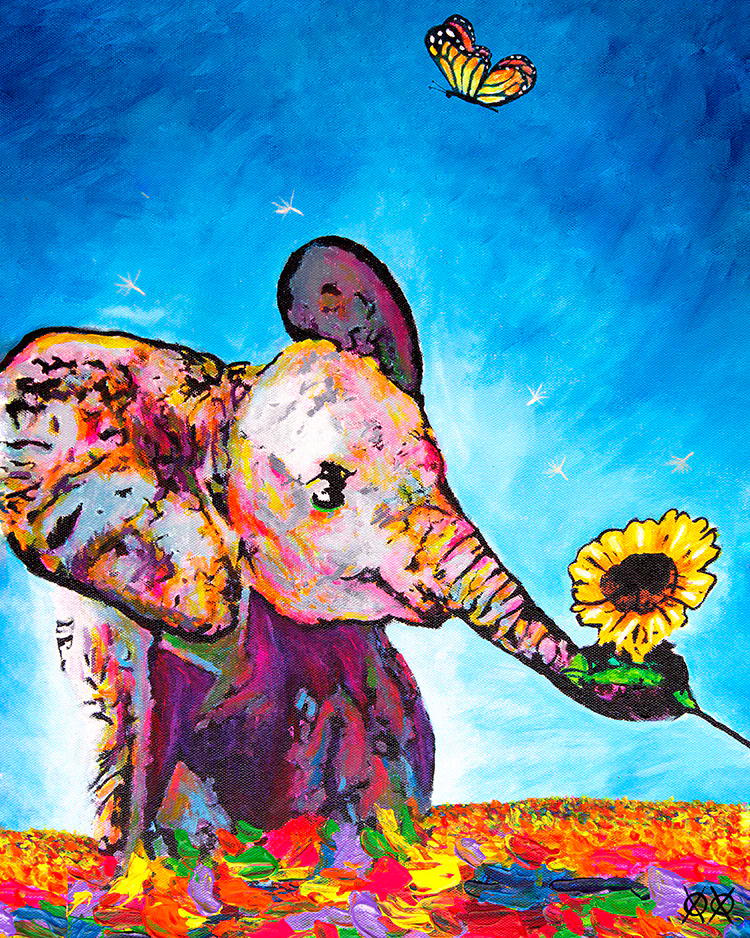
\includegraphics[width=15mm]{elephant.png}
  \end{wrapfigure}
\end{verbatim}
ce qui n'est pas si difficile comme on a tendance de croire. Je peux même vous
dire que j'ai fini tout ça dans un endroit tellement bruyant que normalement
on aurait du mal à faire qqch de difficile. [J'ai ajouté cette dernière phrase
sous prétexte de rendre le paragraphe plus long.]




\end{document}
